% !TEX program = pdflatex
\documentclass[11pt,a4paper]{article}

% --- packages (kept minimal and standard) ---
\usepackage[utf8]{inputenc}
\usepackage[T1]{fontenc}
\usepackage{lmodern}
\usepackage{geometry}
\geometry{margin=1in}
\usepackage{amsmath,amssymb}
\usepackage{siunitx}
\usepackage{graphicx}
\usepackage[font=small,labelfont=bf,labelsep=endash]{caption}
\usepackage{booktabs}
\usepackage{physics}
\usepackage{hyperref}
\hypersetup{colorlinks=true,linkcolor=blue,citecolor=blue,urlcolor=blue}

% --- title & author ---
\title{Design Methodology for a Dual-Jet Hovering Disc Using Concentric Air Curtains}
\author{ }
\date{ }

\begin{document}
\maketitle

\begin{abstract}
This work presents a physical model and an operational design methodology for a hovering disc sustained by two concentric air jets. The outer annular jet forms an aerodynamic curtain that confines the inner flow and minimizes leakage, whereas the inner jet compensates the residual mass loss to maintain a controlled cushion pressure beneath the disc. Unlike thin-film or incompressible assumptions, the analysis adopts a low-Mach \emph{compressible}, axisymmetric model over a finite-height domain with height comparable to radius. The governing equations for lift, leakage, and curtain dynamics are stated together with boundary conditions that \emph{explicitly enforce a purely vertical outer jet at the upper plane} $z=h$ on the annulus $R^-\le r\le R_{\text{tot}}$. An algorithm is provided to compute pressure and velocity fields over the entire $(r,z)$ domain to achieve stable hovering with minimal power.
\end{abstract}

\section{Introduction and Operating Principle}
The device is a rigid circular disc of total radius $R_{\text{tot}}$ hovering at a distance $h$ from the ground by sustaining an overpressure $p_c$ in the central region. Two coaxial jets are employed (Fig.~\ref{fig:geometry}): an \emph{outer annular jet} (``corona'') acting as an air curtain that seals and recirculates the cushion flow, and an \emph{inner jet} that compensates residual mass leakage across the periphery. The design objective is to select geometry and jet operating points so that the target payload $W$ is carried with acceptable power and stability margins.

\section{Assumptions and Computational Domain}
We explicitly state the assumptions used throughout the model:
\begin{itemize}
  \item \textbf{Axisymmetry.} The flow is axisymmetric with no swirl. The computational domain is the \emph{positive half-plane} $(r\ge 0,\, z\ge 0)$.
  \item \textbf{Finite-height, no thin-film hypothesis.} Height and radius are \emph{comparable}: $h \sim R_{\text{tot}}$; no $h\ll R$ assumption is made.
  \item \textbf{Compressible, low-Mach gas.} Air obeys $p=\rho R_g T$, with Mach numbers sufficiently low to avoid shocks, while allowing density and temperature variations.
  \item \textbf{No solid inside the domain.} In $r\in[0,R_{\text{tot}}]$, $z\in[0,h]$ there are \emph{no solid obstacles}: the whole volume is air at different $(p,T,\mathbf{v})$. The \emph{boundaries} are the ground ($z=0$), the disc underside ($z=h$), the axis ($r=0$), and the outer radial boundary ($r=R_{\text{tot}}$).
  \item \textbf{Outer jet: purely vertical at the top plane.} At $z=h$ and on the annulus $R^-\le r\le R_{\text{tot}}$ the outer jet issues \emph{purely vertical}: $u(r,h)=0$, $w(r,h)=-U_{\mathrm{corona}}$ (\S\ref{subsec:vertical-jet}).
  \item \textbf{Leakage ring.} The leakage annulus has width $w$ so that the inner “core’’ extends to $R^-=R_{\text{tot}}-w$.
  \item \textbf{Steady, mean flow.} The analysis targets mean fields; acoustic fluctuations are neglected.
\end{itemize}

\section{Geometry and Notation}
We adopt the following notation, consistent with the schematic in Fig.~\ref{fig:geometry}:
\begin{itemize}
  \item $R_{\text{tot}}$ total radius; $R^-=R_{\text{tot}}-w$ inner edge of the leakage annulus of width $w$;
  \item $h$ nominal clearance to the ground; $p_c$ target cushion overpressure (area-averaged); $W$ payload;
  \item Outer jet (\textit{corona}): mass flow $\dot m_{\mathrm{corona}}$, slot thickness $b$, slot area $A_{\mathrm{corona}}=2\pi R_{\text{tot}}\,b$, exit speed $U_{\mathrm{corona}}=\dot m_{\mathrm{corona}}/(\rho_j A_{\mathrm{corona}})$ with jet density $\rho_j$;
  \item Inner jet: mass flow $\dot m_{\mathrm{in}}$ (fills residual losses);
  \item Mass loss across the periphery: $\dot m_{\mathrm{loss}}$; volumetric loss $Q_{\mathrm{loss}}=\dot m_{\mathrm{loss}}/\rho_\mathrm{edge}$ with $\rho_\mathrm{edge}=\rho\!\big(p_\mathrm{edge},T_\mathrm{edge}\big)$.
\end{itemize}

\begin{figure}[t]
  \centering
  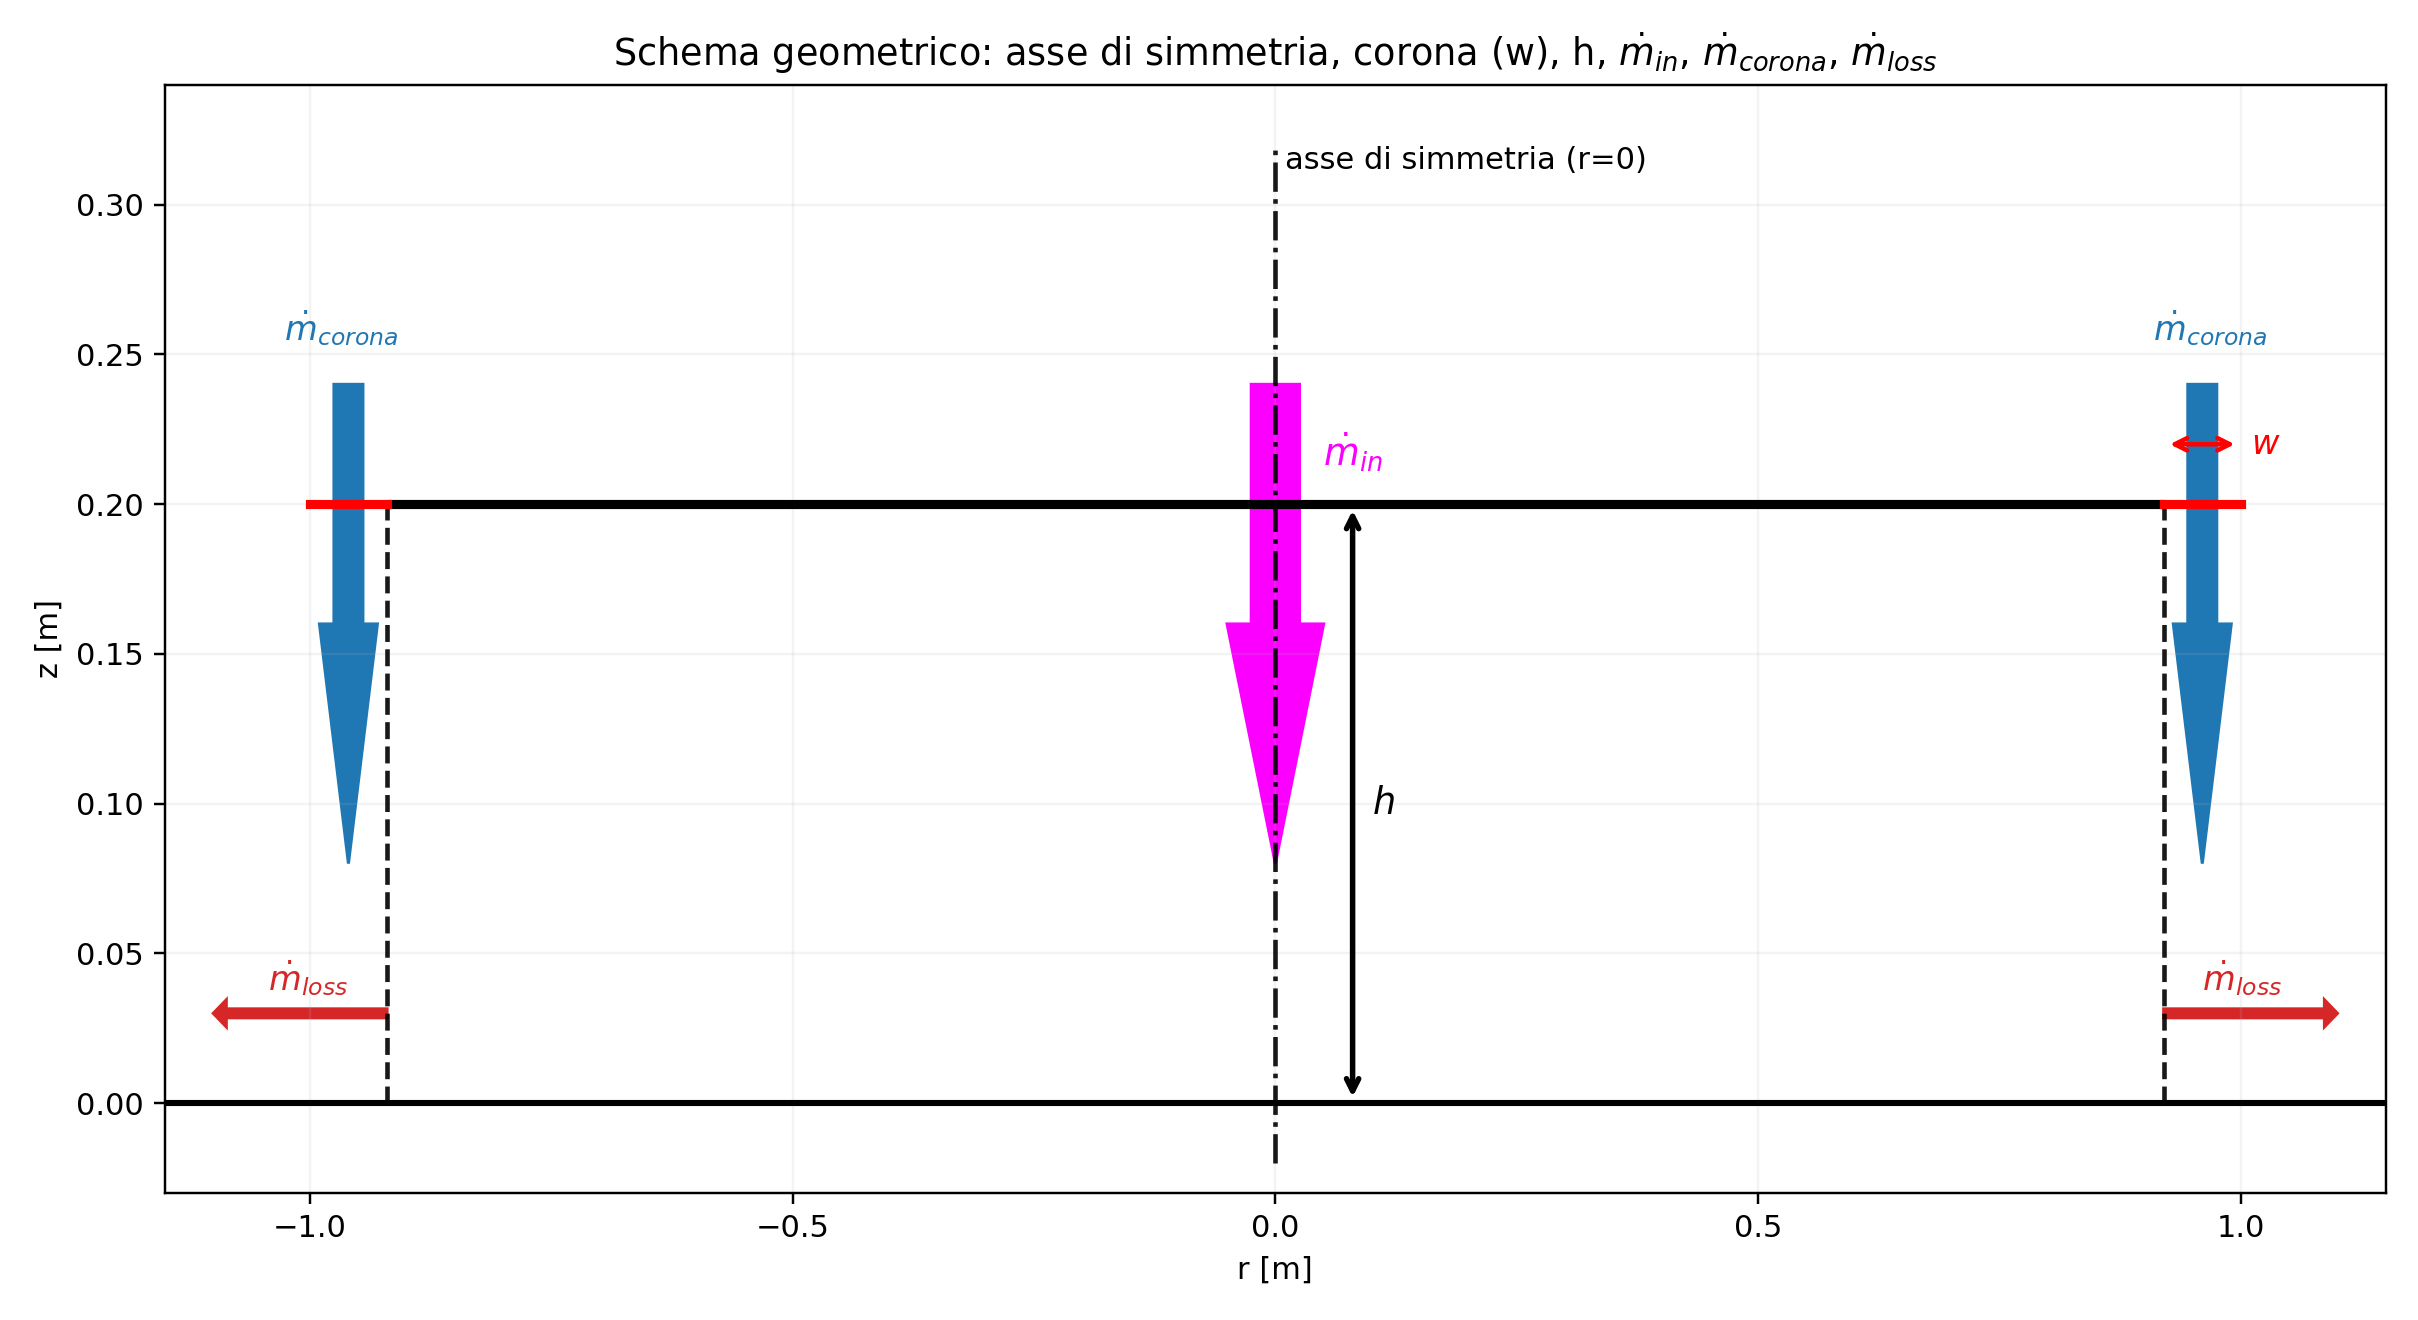
\includegraphics[width=0.95\linewidth]{./figures/schema_geometry.png}
  \caption{Geometric scheme: domain $(r,z)\in[0,R_{\text{tot}}]\times[0,h]$, annulus width $w$, hover height $h$, and the two concentric jets. The outer annular jet is \emph{purely vertical at $z=h$} on $R^-\!\le r\!\le R_{\text{tot}}$, then turns near the ground forming the air curtain that reduces leakage $\dot m_{\mathrm{loss}}$; the inner jet compensates the residual mass loss.}
  \label{fig:geometry}
\end{figure}

\section{Lift Balance}
\begin{equation}
  p_c\,\pi R_{\text{tot}}^2 = W
  \quad \Rightarrow \quad
  p_c = \frac{W}{\pi R_{\text{tot}}^2}.
  \label{eq:lift}
\end{equation}

\section{Leakage Through the Peripheral Gap}
The peripheral annulus governs the mass loss $\dot m_{\mathrm{loss}}$. Select the regime by $\mathrm{Re}_h=\rho_\mathrm{edge} U_h h_{\mathrm{eff}}/\mu$, with $U_h\approx Q_{\mathrm{loss}}/(2\pi R_{\text{tot}} h_{\mathrm{eff}})$.
\subsection*{Viscous (lubrication) regime}
\begin{equation}
  Q_{\mathrm{loss}}
  = \frac{\pi h_{\mathrm{eff}}^{3}\,\big(p_\mathrm{edge}-p_0\big)}{6\,\mu\,\ln\!\big(\tfrac{R_{\text{tot}}}{R_{\text{tot}}-w}\big)},
  \qquad \dot m_{\mathrm{loss}}=\rho_\mathrm{edge}\,Q_{\mathrm{loss}}.
  \label{eq:qloss_lub}
\end{equation}
\subsection*{Inertial (orifice) regime}
Let $A_{\mathrm{eff}}=2\pi R_{\text{tot}}\,h_{\mathrm{eff}}$:
\begin{equation}
  Q_{\mathrm{loss}}
  = C_d\,A_{\mathrm{eff}}\,\sqrt{\frac{2\,\big(p_\mathrm{edge}-p_0\big)}{\rho_\mathrm{edge}}},
  \qquad \dot m_{\mathrm{loss}}=\rho_\mathrm{edge}\,Q_{\mathrm{loss}}.
  \label{eq:qloss_orif}
\end{equation}

\section{Outer Air-Curtain Dynamics}
\subsection{Vertical corona jet at \texorpdfstring{$z=h$}{z=h}}
\label{subsec:vertical-jet}
The outer jet issues \emph{purely vertical} at the top plane:
\begin{equation}
  \boxed{ \ u(r,h)=0,\qquad w(r,h)=-U_{\mathrm{corona}},\qquad R^-\le r\le R_{\text{tot}} \ }.
  \label{eq:verticalBC}
\end{equation}
This kinematic condition is the physical inlet for the corona. The jet then turns near the ground forming a wall-jet that exerts a sealing action on the rim.

\subsection{Sealing (pressure) condition at the rim}
A momentum balance for the turned jet yields the pressure distribution applied at the inner rim $r=R^-$:
\begin{equation}
  \boxed{\
  p_\mathrm{edge}(z) \;=\; p_0 \;+\;
  C_t\,\frac{\rho_j U_{\mathrm{corona}}^{2}\,b}{h_{\mathrm{eff}}}\,\phi\!\left(\frac{z}{h}\right),
  \qquad 0\le z\le h \ }.
  \label{eq:curtain_force}
\end{equation}
Because the jet is vertical at $z=h$, most of the effective sealing is delivered \emph{near the ground}; accordingly, we adopt a profile
\begin{equation}
  \phi(\zeta)=(1-\zeta)^{m},\qquad m\in[1,2],
  \label{eq:phi}
\end{equation}
so that $\phi(0)=1$ (max near the ground) and $\phi(1)=0$ (negligible near the top). The momentum ratio reads
\begin{equation}
  J \;\equiv\; \frac{\rho_j U_{\mathrm{corona}}^{2}\,b}{(p_c-p_0)\,h_{\mathrm{eff}}}
  \qquad\Rightarrow\qquad J\gtrsim J_{\min}=1/C_t,
  \label{eq:J}
\end{equation}
and the curtain mass flow is
\begin{equation}
  \dot m_{\mathrm{corona}} = \rho_j\,A_{\mathrm{corona}}\,U_{\mathrm{corona}}
  = 2\pi R_{\text{tot}}\,\rho_j\,b\,U_{\mathrm{corona}}.
  \label{eq:mcorona}
\end{equation}
The inward fraction $\beta$ of the turned jet that reinforces the core is parameterized as
\begin{equation}
  \beta = \frac{1}{1+\gamma\,(h_{\mathrm{eff}}/b)\,J^{-1/2}},\qquad \gamma=\mathcal{O}(1).
  \label{eq:beta}
\end{equation}

\section{Core Model: Compressible, Axisymmetric, Finite Height}
We model the core region $0\le r\le R^-, 0\le z\le h$ with a low-Mach compressible flow (no swirl). For a fast design-oriented solve we adopt an \emph{anisotropic Stokes--Darcy closure} for mean velocities:
\begin{equation}
  u = -\frac{\kappa_r}{\mu}\,\partial_r p,\qquad
  w = -\frac{\kappa_z}{\mu}\,\partial_z p,
  \qquad \kappa_r=\alpha_r h^2,\ \kappa_z=\alpha_z h^2.
  \label{eq:darcy}
\end{equation}
Combining with continuity for $\rho(p,T)=p/(R_g T)$ gives the elliptic problem
\begin{equation}
  \frac{1}{r}\,\partial_r\!\big(r\,\rho\,\kappa_r\,\partial_r p\big)+\partial_z\!\big(\rho\,\kappa_z\,\partial_z p\big)=0
  \quad\text{in}\quad (r,z)\in[0,R^-]\times[0,h].
  \label{eq:elliptic}
\end{equation}

\paragraph{Boundary conditions (core).}
\begin{itemize}
  \item Axis $r=0$: symmetry, $\partial_r p=0$, $\partial_r T=0$.
  \item Ground $z=0$ and disc underside $z=h$ (over the core): no normal flow for the Darcy closure ($w=0\Rightarrow \partial_z p=0$). Thermal exchange via
  $-k\,\partial_n T=h_0\,(T-T_{s0})$ at $z=0$ and $-k\,\partial_n T=h_1\,(T-T_{s1})$ at $z=h$.
  \item Rim $r=R^-$: \emph{pressure prescribed} by the sealing condition \eqref{eq:curtain_force}.
\end{itemize}

\paragraph{Remark (full-domain alternative).}
If one solves the full axisymmetric Navier--Stokes over $0\le r\le R_{\text{tot}}$, then the \emph{kinematic} boundary condition \eqref{eq:verticalBC} is imposed explicitly on $R^-\le r\le R_{\text{tot}}$ at $z=h$ (with $u=0$, $w=-U_{\mathrm{corona}}$), while the rim condition \eqref{eq:curtain_force} is no longer needed as a Dirichlet pressure at $r=R^-$ (it emerges from the momentum balance of the turned jet).

\section{Cushion Mass Balance and Make-Up Flow}
\begin{equation}
  \dot m_{\mathrm{in}} + \dot m_{\mathrm{rein}} = \dot m_{\mathrm{loss}}
  \quad\Rightarrow\quad
  \boxed{\ \dot m_{\mathrm{in}} = \dot m_{\mathrm{loss}} - \beta\,\dot m_{\mathrm{corona}}\ }.
  \label{eq:massbalance}
\end{equation}

\section{Power Estimates}
\begin{equation}
  P_{\mathrm{ideal}} \approx p_c\,Q_{\mathrm{loss}} + \frac{\dot m_{\mathrm{corona}}\,U_{\mathrm{corona}}^{2}}{2},
  \qquad P=P_{\mathrm{ideal}}/\eta.
  \label{eq:power}
\end{equation}

\section{Algorithm for $(r,z)$ Fields over $0\!-\!h$ and $0\!-\!R_{\text{tot}}$}
\subsection*{Inputs}
$R_{\text{tot}},\,w,\,h,\,h_{\mathrm{eff}},\,b,\,W,\,\rho_j,\,U_{\mathrm{corona}},\,T_j,\,T_\infty,\,C_t,\,m,\,C_d,\,\mu,\,k,\,c_p,\,R_g,\,h_0,\,h_1$; closure parameters $\alpha_r,\alpha_z$.

\subsection*{Option A: Core-only (fast design, Stokes--Darcy)}
\begin{enumerate}
  \item Compute $p_c$ from Eq.~\eqref{eq:lift}.
  \item Set the sealing pressure $p_\mathrm{edge}(z)$ via Eqs.~\eqref{eq:curtain_force}--\eqref{eq:phi} (with jet vertical at $z=h$).
  \item Choose leakage regime and compute $\dot m_{\mathrm{loss}}$ (Eqs.~\eqref{eq:qloss_lub}--\eqref{eq:qloss_orif}).
  \item Solve the elliptic problem \eqref{eq:elliptic} with BCs above; recover $u,w$ from \eqref{eq:darcy}.
  \item Enforce mass balance \eqref{eq:massbalance} to obtain $\dot m_{\mathrm{in}}$; evaluate power \eqref{eq:power}.
\end{enumerate}

\subsection*{Option B: Full domain (explicit vertical jet at $z=h$)}
\begin{enumerate}
  \item Same steps 1--3 as above to size the operating point; then solve the axisymmetric low-Mach Navier--Stokes on $r\in[0,R_{\text{tot}}]$, $z\in[0,h]$ with:
  \begin{itemize}
    \item $u=0$, $w=-U_{\mathrm{corona}}$ on $z=h$, $R^-\le r\le R_{\text{tot}}$ (Eq.~\eqref{eq:verticalBC});
    \item no-slip or Darcy-normal constraints elsewhere on $z=h$ and at $z=0$;
    \item symmetry at $r=0$; suitable far-field at $r=R_{\text{tot}}$ ($p\to p_0$, $T\to T_\infty$).
  \end{itemize}
  \item The rim pressure $p_\mathrm{edge}(z)$ emerges from the numerical solution and can be compared \emph{a posteriori} with Eq.~\eqref{eq:curtain_force} for calibration of $C_t$ and $m$.
\end{enumerate}

\section{Calibration and Design Parameters}
The following lumped parameters are to be validated on the target geometry: (i) the curtain factor $C_t$ and the vertical distribution exponent $m$ in \eqref{eq:phi}, (ii) the inward fraction $\beta$ in \eqref{eq:beta}, (iii) the discharge coefficient $C_d$ for inertial leakage, and (iv) the anisotropic permeabilities $\kappa_r=\alpha_r h^2$, $\kappa_z=\alpha_z h^2$ used in the Stokes--Darcy closure.

\end{document}
